%TEX root = ../dissertation.tex

\chapter{Related Work}
\label{chapter:related_work}

Some systems have been designed to provide more direct support for managing multiple concurrent activities associated with a large amount of digital material and tools.

In the further section, we discuss software for both clinical and non-clinical imaging tools. More specifically, we address image modality concerning medical applications as well as non-medical applications (e.g., surveillance).

Also, we address software concerning the (non)-multimodality views and existing work in the field of medical and clinical user interfaces.

\section{Activity-Based Computing}

In this section we address other approaches like an Activity-Based Computing (ABC) for Medical Work in Hospitals \cite{citeulike:4920996} that presents the concept, which seeks to create computational support for human activities contributing to the growing research on support for human activities, mobility, collaboration, and context-aware computing. To summarise, activity-based computing builds and expands upon prior work within each of the areas described as activity management, virtual window management, collaboration support systems and context-awareness. However the last topics, it does not approach a multimodal view of images, but it was great on other fields of understanding the context and most of the problem/solutions.

\section{Fine Needle Aspirate}

Another direction of work is known as Fine Needle Aspirate (FNA) \cite{ahmad2012breast}. Basically, their class of approaches, by using computer based image analysing, we research a Breast Cytology Diagnosis via Digital Image Analysis \cite{Mangasarian95breastcancer} paper work that brings us an improvement on the diagnostic accuracy of breast FNA goal where an interactive computer system has been developed for evaluating cytologic features derived directly from a digital scan of breast FNA slides. The system uses computer vision technology techniques to analyse cell nuclei and classifies them using an inductive method based on linear programming.

\clearpage

The researched accuracy for medical imaging breast cancer diagnosis from FNAs varies considerably. Reported accuracy for visually diagnosing breast cancer from FNAs varies considerably. Giard and Hermans \cite{Robertson04scalablefabric} researched on FNA performance parameters and found some sensitivities. The FNA diagnosis is highly operator-dependent and emphasised the need for developing individual performance characteristics for those doing this test. One goal of the present work is to improve the diagnostic accuracy of FNA by increasing its objectivity and thereby making it less operator-dependant. This image analysis and machine learning applied to breast cancer diagnosis and prognosis \cite{citeulike:4920996} study introduce us to a breast cancer diagnosis and prognosis by computer and to the value of aspiration cytologic examination of the breast into a statistical review of the medical literature \cite{Robertson04scalablefabric:}.

\section{Picture Archiving and Communication Systems}

Medical services in current-time rely heavily on digital imaging technology due to image modalities utilised in medical field such as the computer Ecography, Mammography and \gls{MRI}. These techniques require image-processing tools and digital management that has been the primary reason for development of Picture Archiving and Communication Systems (PACS) \cite{oosterwijk2004pacs}. This technology provides economical storage and convenient access to images from multiple modalities where images are transmitted digitally via PACS where it eliminates the need to manually file, retrieve, or transport film jackets. The universal format for PACS image storage and transfer is Digital Imaging and Communications in Medicine (DICOM) \cite{mustra2008overview} format.

The work that addresses the web based medical images, data processing and management systems, present an application of database and functional imaging \cite{kim2000web} runs through the network and internet browser that has similar ability to the PACS yet having the advantages of being an online system can be viewed as archiving one step closer towards total online medical imaging system and online imaging in general. Despite the excellent information that this paper offer in the field of this research, we are more concerned with analysing the problem in a multimodality shed of image and interface surround, than this distribution of information side.

\section{Computer Aided Diagnosis}

The Picture Archiving and Communication System (PACS) \cite{oosterwijk2004pacs} faces ever-growing adoption in hospitals and clinics worldwide \cite{lemke2003pacs} as we seen before. Digitalisation process and sharing of medical images is progressively replacing the use of tomography films, thus reducing costs and increasing the possibility of remote medical diagnosis through telemedicine solutions. Inline with this trend, Computer Aided Diagnosis (CAD) \cite{giger1993computer} is also gaining ground. CAD is an interdisciplinary technology combining elements of machine learning and computer vision with radiological image processing. A typical application is the detection of a tumor. For instance, some hospitals use CAD to support preventive medical check-ups in mammography (diagnosis of breast cancer). CAD typically intends to provide suggested diagnosis based on automatic quantitative analysis of medical images in order to aid physicians in their final diagnosis.

\clearpage

The output of ML based algorithms may be useful in situations where the human visual system might fail or in case of fatigue of the physicians, alerting on possible well-known problems. According to a computer-aided diagnosis in medical imaging article \cite{giger1993computer}, there are two CAD system types. The first type of CAD system assists with lesion detection, searching for abnormal standards in images like micro-calcifications groups in mammography images. The second type of CAD system assists the diagnosis, analysing the quantification of image characteristics where extracting information about a lesion shape may help to determine if a tumor is malignant or benign.

\section{Patient Visualisation}

A two different interfaces to visualize patient histories on a PDA \cite{ardito2006two} describes two different users interfaces for mobile device tool that displays patient histories and permits to visually query patient data stored in hospital database.

% Commands to include a figure:
\begin{figure}[!hbt]
\centering
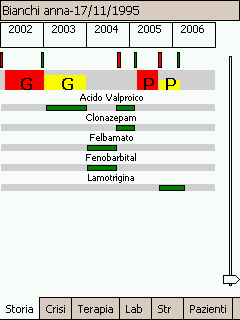
\includegraphics[width=10cm]{images/zoomable}~\\
\caption{\label{fig:zoomable}Zoomable interface of PHiP.
}
\end{figure}

The objective of this work is to display as much as possible information about the patient history on a limited display space, providing overview data as well as details. By displaying on a single screen of a personal computer the overview of multiple facets of records will provide users with a better sense of type and volume of available data.

In fact, PHiP (Patient History in Pocket) \cite{ardito2006two} is a tool designed for a mobile device that displays patient histories and permits to visually query patient data stored in the hospital database exploiting information visualisation techniques where it is able to accommodate on the screen a good amount of clinical cases.

This work has been developed according to an user-centered approach and will bring MIMBCD-UI support in that way. Beside the user studies conducted in the hospital at the requirement phase, they have performed with doctors evaluations of the different prototypes and this kind of information is kindly useful for our research field as well.

\section{Patient Progress}

In computer-assisted creation of patient progress notes \cite{wilcox2009activenotes} a prototype application that supports the creation of critical care notes by physicians in a hospital of an intensive care unit, called activeNotes, integrates automated, context-sensitive patient data retrieval and user control of automated data updates and alerts into the note creation process.

% Commands to include a figure:
\begin{figure}[!hbt]
\centering
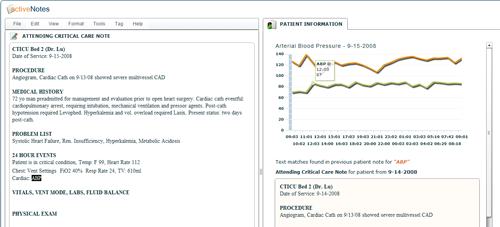
\includegraphics[width=15cm]{images/activenotes}~\\
\caption{\label{fig:activenotes}activeNotes Prototype System.
}
\end{figure}

A critical care note is a clinical document, written by a hospital physician, that documents and patient's progress and prognosis. This kind of work will help MIMBCD-UI project by giving us information analyse by physicians feedback and user understanding. It also bring us information with qualitative study by providing us the right path throw prototype design and user experience evaluation.

The physician-driven management of patient progress notes in an intensive care unit [20], describes a design exploration focused on techniques to support data input and management of electronic progress note content. This will help MIMBCD-UI project by giving us an alternative design exploration including observations, structured and semi-structured interviews, design and implementation of a prototype, and feedback gathered in qualitative study with physicians surveys.

\section{Interaction System}

On M/ORIS: a Medical/Operating Room Interaction System \cite{grange2004m} is proposed an architecture for a real-time multimodal system, which provides non-contact, adaptive user interfacing for Computer-Assisted Surgery (CAS) \cite{hahn2001visualization}. This paper focuses on the proposed activity monitoring aspects of M/ORIS. The researchers have analyse the issues of Human-Computer Interaction (HCI) in an Operation Room (OR) based on real-world case studies.

% Commands to include a figure:
\begin{figure}[!hbt]
\centering
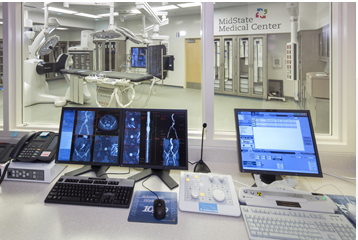
\includegraphics[width=15cm]{images/moris}~\\
\caption{\label{fig:moris}Operating room interaction system example.
}
\end{figure}

\subsection{CAS vs CAD}

Computer Aided Surgery (CAS) \cite{wikipedia2016computerassisted} and Computer Aided Diagnosis (CAD) \cite{wikipedia2016computeraided} can contribute to the general cost cutting trend in health care by making it possible to have fewer staff perform the same activity in less time than with traditional methods. It also brings us human error prevention and, if so, the system can better audit the source of problems and reduce error effects. In particular, it is likely that in the near future, a single doctor will have to control and diagnose several computer-based processes during a surgical, diagnosis or clinical intervention.

Efficient User Interface (UI) design that matches the constrains of clinical environments and that helps reduce the doctor's workload will, in a large part, determine the success of CAS and CAD.

\subsection{User Interface for CAD}

The impressive development of medical multimodality of imaging technology during the last decades provided physicians with an increasing amount of patient functional data and specific anatomical. Furthermore, the increasing use of non-ionising real-time imaging, in particular optical and ultrasound imaging, during cancer analysing procedures created the need for design and development of new visualisation of information and display technology \cite{sielhorst2008advanced} allowing physicians to take full advantage of rich sources of heterogeneous preoperative and intra-operative data. The medical augmented reality was proposed as a paradigm bringing new visualisation and interaction solutions into perspective.

\clearpage

CAD techniques, whether they enhance traditional methods (e.g. image visualisation \cite{vogt2003system}) or provide new tools such as augmented displays \cite{sielhorst2008advanced}, share a common need for multimodality of imaging \gls{UI}. Interface issues are systematically brought up in connection with new computer-assisted techniques, and poor UI design is cited \cite{grange2004m, vogt2003system} as significant limiting factor for many operations. In particular, doctors criticise the lack of user-centered design, the difficulty to operate computer-assisted equipment during surgery, and the failure to convey information without otherwise constraining the doctor.

To address these issues, several authors have developed guidelines for medical UI design. An introduction to human factors in medical devices \cite{sawyer1996introduction} and making medical device interfaces more user-friendly \cite{wiklund1998making} stress the importance of a doctor-centered design for both efficiency and human error reduction. A framework for determining component and overall accuracy for computer assisted surgery systems \cite{mor2003framework} proposes a framework for evaluating the benefits of new UI paradigms in CAS system design that can be applied to CAD system design.

\section{Designing the User Interface}

Multimodal systems that process user's speech and pen-based gestural input have become a vital and expanding field, especially within the past years, with demonstrated advances in a growing number of research and application areas.

A growing interest in multimodal interface design is inspired in large part by the goals of supporting more transparent, flexible, efficient and powerfully expressive means of human-computer interaction that in the past. Multimodal interfaces are expected to support a wider range of diverse applications, be usable by a boarder spectrum of the average population, and function more reliably under realistic and challenging usage conditions.

In designing the user interface for multimodal speech and pen-based gesture applications: state-of-the-art systems and future research directions \cite{oviatt2000designing} article, researchers summarise the prevailing and emerging architectural approaches available for interpreting dual input signals in a robust manner, including early and late semantic fusion approaches, as well as new hybrid symbolic-statistical architecture, that potentially are capable of archiving very robust functioning, for processing pen-voice input (i.e. speech and gesture). Researchers also described a diverse collection od state-of-the-art multimodal systems that are capable of processing user's actions input. This will brings an enormous added value in the implementation and architecture of our future user interface.

\section{Usability and Ergonomic Testing}

Semiotic analysis combined with usability and ergonomic testing for evaluation of icons in medical user interface \cite{bhutkar2011semiotic} have evaluated the medical icons and iconic interfaces of touch screen ventilator systems used in Intensive Care Unit (ICU).

The use of icons in iconic user interfaces \cite{katre2004experimenting} in medical devices like ventilator systems is a common practice. Precise communications through iconic interface between ventilator system and medical users like physicians or nurses is critical to avoid medical errors which may cost patient's life.

This research will help us understand and defining a set of icons that will represent our metaphor analysis throw this work. It also, but not less, give us the right information about usability testing where icons can be tested using various usability testing methods. At last it will help us getting information about Semiotic and Lexical Analysis.

Semiotics is a study of cultural sign processes, analogy, signification, communication, metaphors, signs and symbols \cite{semiotics}. A semiotic analysis is concerned with meaning, which stems from relationships - in particular, the among signs relationships \cite{berger2010final}.

Linguistics has a term - 'Lexical Analysis' which is the process of converting a sequence of characters into a sequence of tokens. A lexical analysis helped in classification of medical icons \cite{poovaiah1997graphics} into mainly three classes: icons, indices and symbols.